%%%%%%%%%%%%%% Notes %%%%%%%%%%%%%%%%%%%%%%%%%%%
%1. Tell that you did phase 3 and thus completed this thing.
%2. Tell that in docs, you added register allocation algo, etc.
%%%%%%%%%%%%%%%%%%%%%%%%%%%%%%%%%%%%%%%%%%%%%%%%
%%%%%%%%%%%%%%%%%%%%%%%%%%%%%%%%%%%%%%%%%%%%%%%%
%%%%%%%%%%%%%%%%%%%%%%%%%%%%%%%%%%%%%%%%%%%%%%%%


\documentclass{beamer}

\usepackage{xcolor}  
\usepackage{environ}
\usepackage{minted}
\usepackage{tikzsymbols}
\usepackage[export]{adjustbox}
\usepackage{subcaption}

\hypersetup{
  colorlinks = true,
  linkcolor = blue,
  urlcolor  = blue,
  citecolor = blue,
  anchorcolor = blue
}


% map defaulf block to oldblock
\let\oldblock\block
\let\endoldblock\endblock

% change block by adding smallskip
\renewenvironment{block}[1]
    {\begin{oldblock}{#1}
        \smallskip
    }
    { 
    \end{oldblock}
    }

\usetheme[]{metropolis}

\makeatletter
\setlength{\metropolis@titleseparator@linewidth}{2pt}
\setlength{\metropolis@progressonsectionpage@linewidth}{2pt}
\setlength{\metropolis@progressinheadfoot@linewidth}{2pt}
\makeatother

\newcommand{\iph}[2]{
    \includegraphics[width=#1\textwidth,height=#1\textheight,keepaspectratio]{#2}
}
\newcommand{\ph}[1]{
    \includegraphics[width=0.5\textwidth,height=0.5\textheight,keepaspectratio]{#1}
}

\title{Tiger to RISC V Compiler}

\author{Sourabh Aggarwal\\ Mentor: Dr. Piyush P. Kurur}

\institute[IIT Palakkad] % (optional, but mostly needed)
{
  Department of Computer Science And Engineering\\
  IIT Palakkad
}

\date{November 2019}

\subject{BTP Presentation}

\setminted{breaklines=true, tabsize=2, breaksymbolleft=, fontsize=\footnotesize}

%% Adding color

\definecolor{BlueTOL}{HTML}{6609F5} % or 204FE2
\definecolor{BrownTOL}{HTML}{666633}
\definecolor{GreenTOL}{HTML}{225522}
\definecolor{White}{HTML}{FFFFFF}

\setbeamercolor{title separator}{fg=BlueTOL}
\setbeamercolor{frametitle}{bg=BlueTOL, fg=White}
\setbeamercolor{palette primary}{bg=BlueTOL, fg=White}

\newcommand{\ft}[1]{
  \frametitle{
\includegraphics[height=0.55cm, width=0.55cm, keepaspectratio]{assets/tiger.png} #1}
}

\newcounter{saveenumi}
\newcommand{\seti}{\setcounter{saveenumi}{\value{enumi}}}
\newcommand{\conti}{\setcounter{enumi}{\value{saveenumi}}}

\begin{document}

\begin{frame}
  \titlepage
\end{frame}

\begin{frame}[fragile]
  \ft{What Has Been Acheived}
  \begin{enumerate}
    \item Successfully translated compiler functionality from MIPS to RISC V.
    \begin{enumerate} 
      \item During this process, lots of code refactoring is done along with improvement in time complexity of various intermediate computations. 
      \item Files such as \href{https://github.com/sourabh2311/btp/blob/master/Compiler/runtime.s}{runtime.s} and \href{https://github.com/sourabh2311/btp/blob/master/Compiler/riscframe.sml}{riscframe.sml} were completely rewritten along with various modifications required at other places.
    \end{enumerate}
      \seti
  \end{enumerate}
\end{frame}

\begin{frame}[fragile]
  \ft{What Has Been Acheived}
  \begin{enumerate}
    \conti
    \item Implemented improvements in lexical phase to detect more errors; errors in lexical phase are reported immediately resulting in program termination unlike in semantic analysis where a guess is made to facilitate printing all errors in the end.
    \begin{figure}
    \centering
    \iph{0.80}{assets/lexError.png}
    \label{fig:lexError}
    \end{figure}
    \seti
  \end{enumerate}
\end{frame}

\begin{frame}[fragile]
  \ft{What Has Been Acheived}
  \begin{enumerate}
    \conti
    \item Wrote complete documentation of my compiler at \href{https://tigercompiler.ml}{tigercompiler.ml}. This is done to help me and anyone interested in this project to quickly revise the fundamentals and understand the working of this compiler.
    \begin{figure}
    \centering
    \iph{0.80}{assets/tigercompiler.png}
    \label{fig:tigercompiler}
    \end{figure}
    \seti
  \end{enumerate}
\end{frame}

\begin{frame}[fragile]
  \ft{What Has Been Acheived}
  \begin{enumerate}
    \conti
    \item Wrote automated testing using \href{https://travis-ci.org/sourabh2311/btp}{Travis}. Now I'll be able to see whether my changes don't break the existing functionalities and also it is useful in case someone sends a pull request.
    \begin{figure}
    \centering
    \iph{0.80}{assets/travis.png}
    \label{fig:travis}
    \end{figure}
    \seti
  \end{enumerate}
\end{frame}

\begin{frame}[fragile]
  \ft{What Has Been Acheived}
  \begin{enumerate}
    \conti
    \item \textbf{Fixed} a major bug; Initially my compiler supported only fixed number of arguments. Now this has been extended to support any number of arguments. 
    \begin{figure}
    \centering
    \iph{0.80}{assets/funargs.png}
    \label{fig:funargs}
    \end{figure}
    \begin{figure}
    \centering
    \iph{0.80}{assets/gitfunargs.png}
    \label{fig:gitfunargs}
    \end{figure}
    \seti
  \end{enumerate}
\end{frame}

\begin{frame}[fragile]
  \ft{What Has Been Acheived}
  \begin{enumerate}
    \conti
    \item Added 2 more arithmetic operations, viz. \texttt{left shift} and \texttt{right shift}. 
    \begin{figure}
    \centering
    \iph{0.80}{assets/shiftoperations.png}
    \label{fig:shiftoperations}
    \end{figure}
    \seti
  \end{enumerate}
\end{frame}

\begin{frame}[fragile]
  \ft{What Has Been Acheived}
  \begin{enumerate}
    \conti
    \item Implemented multiplication by power of 2 optimization inside basic block thus laid foundation for other basic block optimizations like constant propagation, constant folding.
    \begin{figure}[t!]
      \centering
      \begin{subfigure}[t]{\textwidth}
      \centering
      \iph{0.80}{assets/mulopt1.png}
      \label{fig:mulopt1}
      \end{subfigure}
      \begin{subfigure}[t]{0.8\textwidth}
      \centering
      % 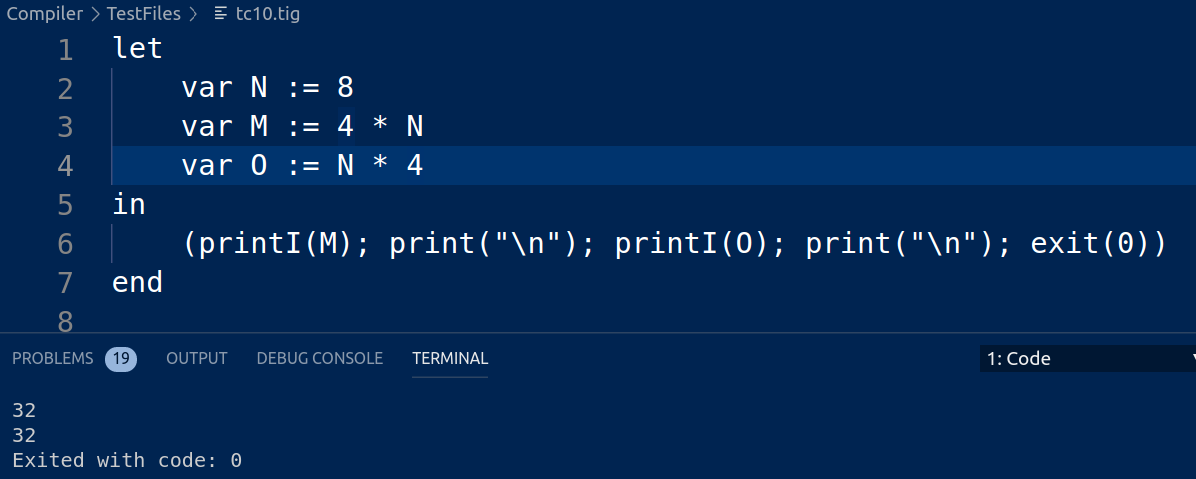
\includegraphics[width=50mm]{assets/mulopt1.png}
      \iph{0.70}{assets/mulopt2.png}
      \label{fig:mulopt2}
      \end{subfigure}
    \end{figure}
    \seti
  \end{enumerate}
\end{frame}

\begin{frame}[fragile]
  \ft{What Has Been Acheived}
  \begin{enumerate}
    \conti
    \item Started work on giving a guess of literal in case of small typo. 
  \begin{itemize}
    \item Printing suggestions which are atmost 2 \href{https://en.wikipedia.org/wiki/Edit_distance}{distance} apart. This will bring the time complexity of standard DP approach of $O(n^2)$ to just $O(n)$. 
    \item Currently the issue is that to implement this, I would have to do lots of modification of the current code. Although I have \href{https://github.com/sourabh2311/btp/commit/8f27478a3c51b9e41bef68961a28c400d4ef29dd}{abstracted} out \textit{Not Found} error messages out with the environment, what is just left is to compare the literal with those of nearby length in the environment. 
    % \item But to efficiently get those strings of nearby length there should be a map which maps lengths to the string set. (An array indexed by length may as well be used) To do this, I would have to define additional data structures and put them at appropriate place. 
    \item The main issue is that in the current design, environment just have integers mapped to environment entry. We got this integer by mapping string to counter, not storing the reverse map. This can be worked around by using \href{http://www.cs.utah.edu/~mjones/sml-nj-lib/atom.html}{Atom}.  
  \end{itemize}
    \seti
  \end{enumerate}
\end{frame}


\begin{frame}[fragile]
  \ft{What Has Been Acheived}
  \begin{enumerate}
    \conti
    \item Started work on improving my Register Allocator. Current version is a bit simplified version of the algorithm mentioned in the text and is without coalescing.
    \seti
  \end{enumerate}
\end{frame}

\begin{frame}[fragile]
  \ft{Road Ahead}
  \begin{itemize}
    \item Register Allocator as mentioned.
    \item Basic blocks has to optimizations as mentioned.
    \item Error messages improvement in semantic phase as mentioned.
    \item String comparison has to be made as simple as "str1 $>$ str2", etc.,  instead of calling the string comparison functions to determine it.
    \item To implement ability to include pre-written code (header) files.
    \item To implement garbage collection.
    \item To implement dataflow analyses such as reaching definitions and available expressions and use them to implement some of the optimizations. 
    \item To implement first-class function values in Tiger, so that functions can be passed as arguments and returned as results.
    \item Add support for compile time (initial) arguments.
  \end{itemize}
\end{frame}
% \begin{frame}
%   \ft{Goal for this Semester}
%   This semester, I am mainly focusing on:-
%   \begin{itemize}
%     \item Understanding RISC V.
%     \item Recollecting all that was done last semester (3 month gap \Xey). % Reason for using tikzsymbols
%     \item Refactoring, fixing bugs and translating everything to RISC V.
%     \item Writing good documentation of the code for easy recollection.
%     \item Travis script for automated testing.
%     \item And of course, if there is time, I'll work on the previous mentioned issues else they are to be focused on next semester.
%   \end{itemize}
% \end{frame}

% \begin{frame}[fragile]
%   \ft{Compiler Course: Phase I - Building AST}
%   Example:-
%   \begin{minted}{sml}
% | LET decs IN exps END              (
%   A.LetExp({decs = decs, body = A.SeqExp(exps), pos = LETleft})
%   )
%   \end{minted}
%   Included many files, viz. 
%   \begin{itemize}
%     \item parse.sml 
%     \item errormsg.sml 
%     \item tiger.lex 
%     \item table.sml, table.sig 
%     \item symbol.sml 
%     \item tiger.grm, absyn.sml 
%   \end{itemize}
% \end{frame}

% \begin{frame}[fragile]
%   \ft{Compiler Course: Phase II - Building Intermeditate Representation Tree}
%   \begin{minted}{sml}
% datatype stm = SEQ of stm * stm 
%             | LABEL of label 
%             | JUMP of exp * label list 
%             | CJUMP of relop * exp * exp * label * label 
%             | MOVE of exp * exp 
%             | EXP of exp 
% and exp = BINOP of binop * exp * exp 
%             | MEM of exp 
%             | TEMP of Temp.temp 
%             | ESEQ of stm * exp 
%             | NAME of label 
%             | CONST of int 
%             | CALL of exp * exp list 
%   \end{minted}
  
% \end{frame}
% \begin{frame}[fragile]
%   \ft{Compiler Course: Phase II - Building Intermeditate Representation Tree}
%   Included many files, viz. 
%   \begin{itemize}
%     \item types.sml 
%     \item env.sml, env.sig 
%     \item temp.sml, temp.sig 
%     \item findescape.sml 
%     \item tree.sml 
%     \item risc.sml 
%     \item translate.sml 
%     \item semant.sml 
%   \end{itemize}
% \end{frame}

\begin{frame}[standout]
Thanks!
\end{frame}   
\end{document}
